\documentclass[]{report}

% PREAMBLE

% A file like this(called home.tex) could be placed in each latex project folder. 

% This will give the possibility to use modules like this:
% % A file like this(called home.tex) could be placed in each latex project folder. 

% This will give the possibility to use modules like this:
% \input{home} - This is needed to use the \home command
% \input{\home/Modules/Usepackages}
% \input{\home/Modules/ChapterStyle}
% \input{\home/Modules/HeaderAndFooter}

% If you use Github or any other collaborating tool, you should ignore the home.tex file, so that every user could have their own home.tex file.

\newcommand{\home}{C:/Users/Alexander/Documents/GitHub/LaTeX} - This is needed to use the \home command
% \input{\home/Modules/Usepackages}
% \input{\home/Modules/ChapterStyle}
% \input{\home/Modules/HeaderAndFooter}

% If you use Github or any other collaborating tool, you should ignore the home.tex file, so that every user could have their own home.tex file.

\newcommand{\home}{C:/Users/Alexander/Documents/GitHub/LaTeX}
\input{\home/Modules/Usepackages}
\input{\home/Modules/ChapterStyle}
\input{\home/Modules/HeaderAndFooter}
\input{\home/Modules/Paragraph}
\input{\home/Modules/Figure}

% Put into module
\usepackage{bm}
\DeclareMathOperator*{\argmin}{arg\,min}
\DeclareMathOperator*{\argmax}{arg\,max}




%FixMe pakken viser små kommentarer, hvor der skal rettes
%--------------------------------------------------
%Brug med følgende: \fxnote{det her skal uddybes!} 
%Se liste over alle fixMe's: \listoffixmes
%Erstat 'draft' med 'final' for at fjerne alle kommentarer
%--------------------------------------------------
\usepackage[footnote,draft,english,silent,nomargin]{fixme}

% Title Page
\title{TiNONS Project - Speaker Recognition: Appendix}
\author{Kasper Nielsen - 10731 \\ Alexander Rasborg Knudsen - 20107083}



\begin{document}
\maketitle

\listoffixmes
\newpage

\tableofcontents





%!TEX root = Appendix_Main.tex
\chapter{Dataset}
\section{Description}
The data that we use to test individual classification methods in this project consists of recordings from 4 speakers repeatedly saying the numbers 0 through nine.
From this set one speaker was removed, because significantly fewer recordings ware made of this.
Hence the amount of data points less fewer than was desired.

Out of the dataset, 15 utterings of each digit ware selected randomly from each speaker, classified and put into the training set.
Another 5 utterings of each digit from each speaker was then classified ad selected as test set.

The data is sampled at $ 48\ kHz, 16\frac{bits}{sample}  $

The data is provided by \cite{DataSet}

\input{features_app} - DONE ?

% Evaluation method
\chapter{Evaluation of classification methods}
The individual classification methods are evaluated with datasets of varying complexities.
Most notably, with speakers uttering the same single digit ("\textit{ZERO}"), two different digits ("\textit{ZERO}" and "\textit{ONE}"), and ten different digits ("\textit{ZERO}", "\textit{ONE}" through "\textit{NINE}").


To evaluate a classifier, the confusion matrix is an ideal way of doing so.
The confusion matrix can show the classifications sensitivity, precision and accuracy for each class. 
The terms used to describe this is: false positive (\textit{FP}), true positive (\textit{TP}), false negative (\textit{FN}) and true negative (\textit{TN}).
The true terms are classes that are correctly classified and false terms are incorrectly classified.
The sensitivity is the probability of classifying the inputs as class $X$ for a input that are class $X$.
\begin{equation}
\mathtt{sensitivity}(X) = \dfrac{TP_X}{TP_X+\Sigma FN_X}
\label{eq:sensitivity}
\end{equation}
The precision is the probability that the estimate of class $X$ is correct.
\begin{equation}
\mathtt{precision}(X) = \dfrac{TP_X}{TP_X+\Sigma FP_X}
\label{eq:precision}
\end{equation}
The accuracy is the probability that the classification of any given class is correct, where N = total number of tests.
\begin{equation}
\mathtt{accuray}(X) = \dfrac{\Sigma TP_X}{\mathrm{N}}
\label{eq:accuracy}
\end{equation}

\begin{table}[H]                                              
\centering                                                     
\begin{tabular}{|l|c|c|c|c|}                                   
\hline                                                         
  & Speaker Jacob & Speaker Mose & Speaker Simon & Precision [\%] \\
\hline                                                         
Estimate Jacob & 6300.0 & 0.0 & 0.0 & 100.0 \\                 
\hline                                                         
Estimate Mose & 10.0 & 5790.0 & 100.0 & 98.1 \\                
\hline                                                         
Estimate Simon & 600.0 & 1120.0 & 6810.0 & 79.8 \\             
\hline                                                         
Sensitivity [\%] & 91.2 & 83.8 & 98.6 & 91.2 \\                
\hline                                                         
\end{tabular}                                                  
\caption{Example of confusion matrix. GMM classification with 3 speakers and 2 digits spoken}                          
\label{table:Ex_conf}                                       
\end{table}

Above in Table \ref{table:Ex_conf} an example of a confusion matrix in shown.
The far right column shows the precision as calculated with (\ref{eq:precision}), 
the bottom row shows the sensitivity as calculated with (\ref{eq:sensitivity})
and the bottom right field shows the overall accuracy as calculated with (\ref{eq:accuracy}).
This is the way, along with some plots of target vs. estimate, that the results of using various methods for classification will be presented in this project.

The evaluation of classifiers will primarily be based on overall accuracy of the classifier. 



% Linear classifiers - DONE?
\chapter{Linear classification}
In linear classification the decision surfaces are linear functions of the input vector \textbf{b}. 
The decision surfaces are defined by D-1 dimensional hyperplane in the D dimensional input space.
the target of the classification is labelled in the target variable \textbf{t}, using the target values to represent class labels. 
In the case of two-class problems, a single target variable can be represented by $t\in \lbrace 0,1\rbrace$ where $t = 1$ represents class $C_1$ and $t = 0$ represents class $C_2$.
If the is more than 2 classes $(K>2)$, then \textbf{t} is a vector of length K.
For Class $C_j$ the element $t_j$ takes value 1 and all other elements $t_k$ of \textbf{t} are zero.
In this project there are 3 different speakers, $K = 3$ then the target vector for class 3 be $\textbf{t} = (0, 0, 1)^T$.
The value of $t_k$ can be interpret as the probability of the given class being class $C_k$.
To assign each vector \textbf{x} with a specific class, a number of different approaches can used to classify.
One way is using a discriminant function, with a linear predictor $y(\textbf{x},\textbf{w})$ given by the parameter \textbf{w} and the input vector set $\textbf{x}=(x_1,...,x_D)^T$, which is linear. 
The linear discriminant function in its simplest form
\begin{equation}
y(\textbf{x}) = \textbf{w}^T \textbf{x}+w_0
\label{eq:lineDis}
\end{equation}
Where $w_0$ is the bias and \textbf{w} is the weight vector.
The decision boundary corresponds to $y(\textbf{x})=constant$, and hence $\textbf{w}^T \textbf{x}+w_0 = constant$ therefore the decision boundary is a linear function.
\\
The process to apply the linear classifier to the dataset, is described below. 
The result of the linear classifier is evaluated by applying a confusion matrix and calculating the accuracy. 
The linear classifier is applied to the training dataset, containing $N =??$ feature vectors $(\textbf{x}_n)$ and the target vectors $(\textbf{t}_n)$.
The vectors are on the form:
\begin{equation}
\textbf{\tilde{X}}=\left[\textbf{x}_1^T 1\\ \textbf{x}_2^T 1\\ ...\\ \textbf{x}_n^T 1\\  \right], \textbf{T}=\left[\textbf{t}_1^T\\ \textbf{t}_2^T\\ ...\\ \textbf{t}_n^T\\ \right]
\label{eq:linearVectors}  
\end{equation} 

To determine the weight matrix $\textbf{\sim{W}}$:
\begin{equation}
\textbf{\tilde{W}} = \textbf{\tilde{X}}^\dagger \textbf{T} \approx  (\textbf{\tilde{X}}^T\textbf{\tilde{X}}+\textbf{I})^{-1} \textbf{\tilde{X}}^T\textbf{T}
\label{eq:weightVector}  
\end{equation}

The are a problem with the entity $\textbf{\tilde{X}}^T\textbf{\sim{X}}$ having small eigenvalues, the solution is to add the identity matrix in the calculations of the pseudo inverse matrix $\textbf{\tilde{X}}^\dagger$.
This is done as a regularization, which can be seen as a penalty for large values in $\textbf{\sim{W}}$.\\

When $\textbf{\tilde{W}}$ is calculated from the training set, it is tested on the test dataset containing $N = ??$ feature vectors and their corresponding targets. 
The result of this equation
\begin{equation}
\textbf{y}(\textbf{x}) = \textbf{\sim{W}}^{T} \tilde{x}, \tilde{x} = \left[\textbf{x}\\ 1 \right] 
\label{eq:Yclassifier}
\end{equation}
shows the most likely class for each of the given feature vectors. 
The resulting vector is placed in a vector $\textbf{t}_{est}$, which contains the classification and ranges over the three classes ${1,2,3}$. show t estimate \fixme

To evaluate the linear classifier, the confusion matrix is an ideal way of doing so.




% Dimensionality reduction / PCA - DONE ?
\chapter{Dimensionality Reduction}
\section{Theory}

\section{Method}

\section{Results}

\section{Discussion}

\fxnote{Diskuter resultater og evt forbedringer} %Done

% Logistic regression / Propabilistic models - MANGLER 

% Artificial Neural Networks - parametric analysis mangler
\chapter{Artificial Neural Networks}

\section{Theory}
Artificial Neural Networks (ANN) also called multilayer perceptron, can be used as a model for pattern recognition. 
The neural network model is a nonlinear function from a set of input variables $ \left\lbrace x_i \right\rbrace  $ transformed to a set of output variables $ \left\lbrace y_k \right\rbrace  $ controlled by the weight vector \textbf{w}, which is made of adjustable parameters.
The number of hidden units between the input and the output can be adjusted to the dataset, the process is described in the method.

The overall network function for a two layer neural network, takes the form
\begin{equation}
y_k(\mathbf{x},\mathbf{w}) = \sigma \left( \sum_{j=1}^{M} w_{kj}^{(2)} h\left( \sum_{i}^{D} w_{ji}^{(1)} x_i + w_{j0}^{(1)} \right) + w_{k0}^{(2)} \right) 
\label{eq:ANN_overall}
\end{equation}
The superscript (1) and (2) indicates which layer the parameter is in, also shown on the parameters in figure \ref{fig:ANN_fig_theory}. 
Both $ \sigma(\cdot) $ and $ h(\cdot) $ are activation functions, which can be chosen to be either the logistic sigmoid or the tanh function.
The part with $ h(...) $ is in the context of ANN called the hidden units. 
D is the number of inputs, M is the number of hidden units and K is the number of outputs.


  
\begin{figure}[H]
\centering
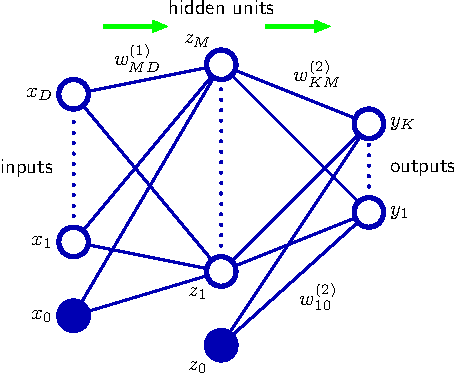
\includegraphics{Figure5_1}
\caption{Diagram of the two layer neural network. The nodes in the figure represents the input, hidden and output variable. The links between the nodes are the weight parameters. The figure is borrowed from \cite{bishop2007}} 
\label{fig:ANN_fig_theory}
\end{figure}

\section{Method}
In both the training and test phases the Netlab Toolbox  was used in MATLAB.
In the training of the neural network for a multi-class classification problem the following error-function is minimized.
\begin{equation}
E(\mathbf{w}) = \dfrac{1}{2} \sum_{n=1}^{N}\| \mathbf{y}(\mathbf{x}_n,\mathbf{w})-\mathbf{t}_n \|^2+\lambda| \mathbf{w}^T \cdot \mathbf{w}|
\label{eq:ANN_error}
\end{equation}
Where $ \mathbf{y}(\mathbf{x}_n,\mathbf{w}) $ is the network function with the parameters and biases in $ \mathbf{w} $ and the target vector, $ \mathbf{t}_n $, is written as a one-of-K-coding.
By minimizing the error-function the parameter that are best for classifying this type of data is fund. 
The parameter include number hidden units and the $\alpha$, which is the inverse variance of the Gaussian noise.
The dataset that was used on the error-function, was the single digit data.
The reason for this, is the vast time it takes to minimizing the error-function, therefore the smallest dataset is used.
This can however make a small error in the number of hidden units optimal for the big dataset of ten digits. 
The number numbers of hidden units found to be optimal is 30, this is used on all of the dataset.

\section{Results}
Using ANN has been tried with different data complexities.
Most notably, with speakers uttering the same single digit ("\textit{ZERO}"), two different digits ("\textit{ZERO}" and "\textit{ONE}"), and ten different digits ("\textit{ZERO}", "\textit{ONE}" through "\textit{NINE}").

\subsection{Single digit:}
\begin{figure}[H]
\centering
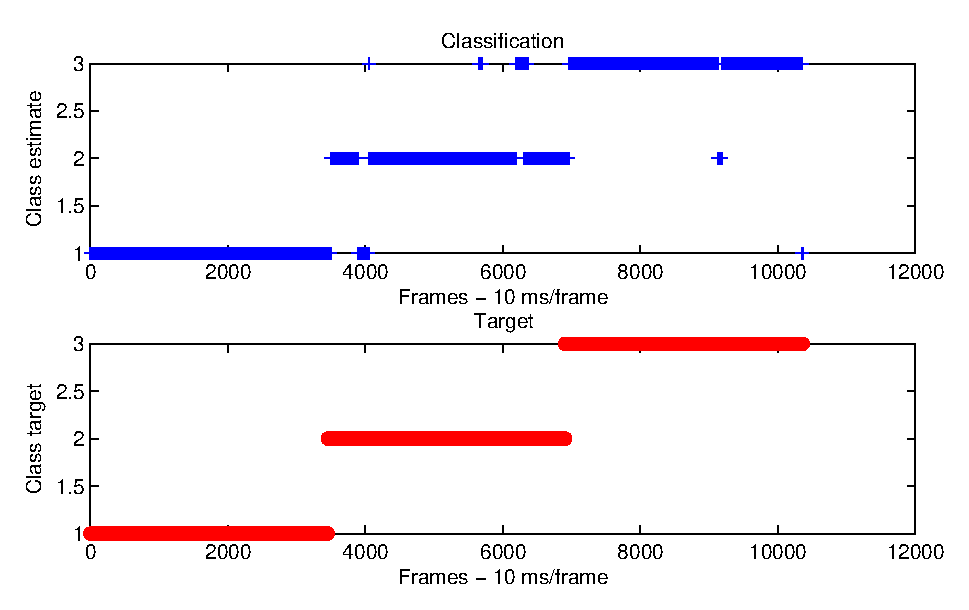
\includegraphics{ANN_1digit_8cent_3speak}
\caption{Results of using ANN with 3 speakers, 30 hidden variables and 1 digit spoken}
\label{fig:ANN_fig_1}
\end{figure}

\begin{table}[H]                                                    
\centering                                                          
\begin{tabular}{|l|c|c|c|c|}                                        
\hline                                                              
  & Speaker Jacob & Speaker Mose & Speaker Simon & Precision [\%] \\
\hline                                                              
Estimate Jacob & 3454.0 & 196.0 & 11.0 & 94.3 \\                    
\hline                                                              
Estimate Mose & 0.0 & 3077.0 & 104.0 & 96.7 \\                      
\hline                                                              
Estimate Simon & 0.0 & 181.0 & 3339.0 & 94.9 \\                     
\hline                                                              
Sensitivity [\%] & 100.0 & 89.1 & 96.7 & 95.3 \\                    
\hline                                                              
\end{tabular}                                                       
\caption{Confusion matrix - 1 digit}                                
\label{table:ANN_conf_1}                                            
\end{table}  



\subsection{Two digits:}
\begin{figure}[H]
\centering
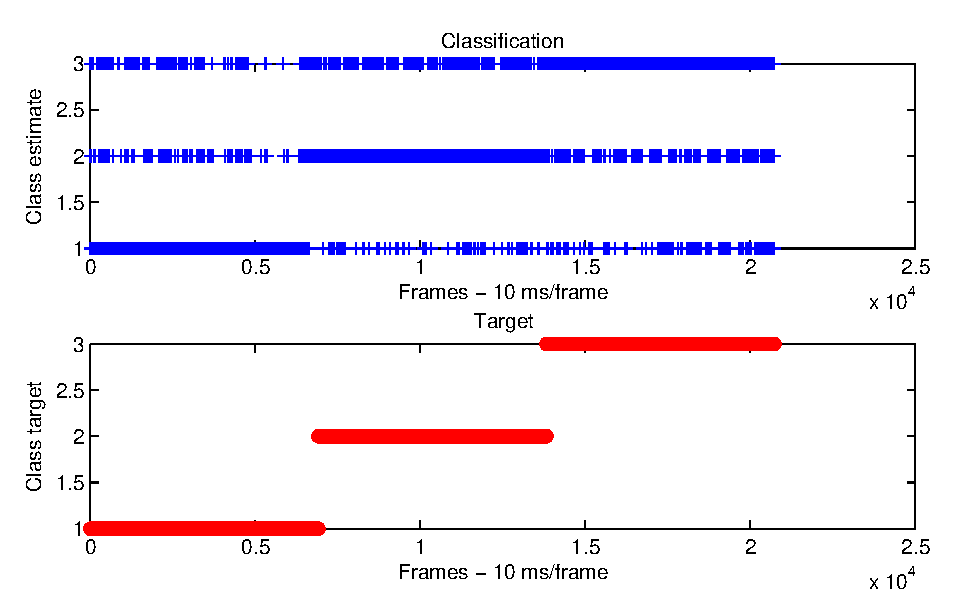
\includegraphics{ANN_2digit_8cent_3speak}
\caption{Results of using ANN with 3 speakers, 30 hidden variables and 2 digits spoken}
\label{fig:ANN_fig_2}
\end{figure}

\begin{table}[H]                                                    
\centering                                                          
\begin{tabular}{|l|c|c|c|c|}                                        
\hline                                                              
  & Speaker Jacob & Speaker Mose & Speaker Simon & Precision [\%] \\
\hline                                                              
Estimate Jacob & 6486.0 & 0.0 & 93.0 & 98.6 \\                      
\hline                                                              
Estimate Mose & 276.0 & 6485.0 & 492.0 & 89.4 \\                    
\hline                                                              
Estimate Simon & 148.0 & 425.0 & 6325.0 & 91.7 \\                   
\hline                                                              
Sensitivity [\%] & 93.9 & 93.8 & 91.5 & 93.1 \\                     
\hline                                                              
\end{tabular}                                                       
\caption{Confusion matrix - 2 digits}                               
\label{table:ANN_conf_2}                                            
\end{table}



\subsection{Ten digits:}
\begin{figure}[H]
\centering
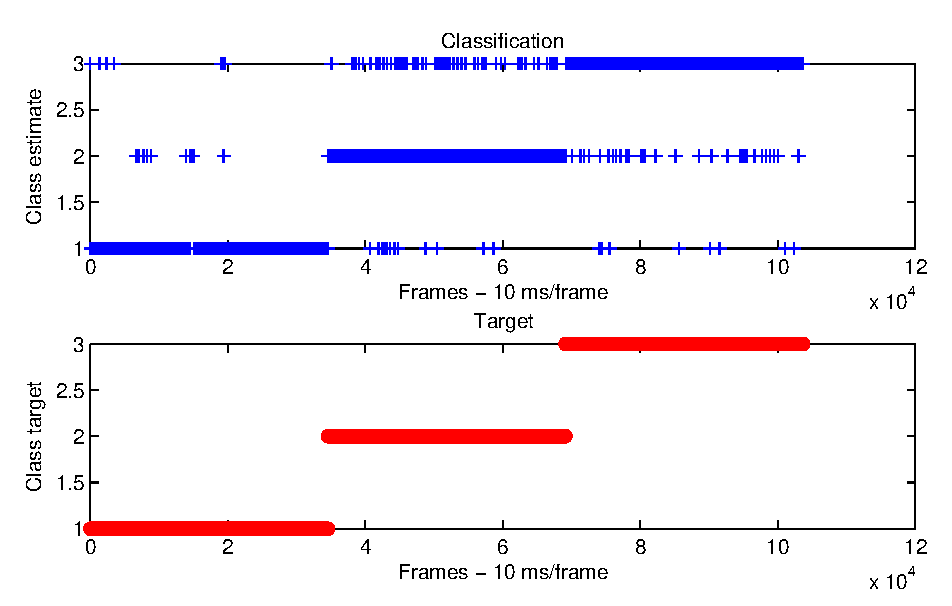
\includegraphics{ANN_10digit_8cent_3speak}
\caption{Results of using ANN with 3 speakers, 30 hidden variables and 10 digits spoken}
\label{fig:ANN_fig_10}
\end{figure}

\begin{table}[H]                                                    
\centering                                                          
\begin{tabular}{|c|c|c|c|c|}                                        
\hline                                                              
  & Speaker Jacob & Speaker Mose & Speaker Simon & Precision [\%] \\
\hline                                                              
Estimate Jacob & 32915.0 & 1186.0 & 528.0 & 95.1 \\                 
\hline                                                              
Estimate Mose & 1245.0 & 28807.0 & 3100.0 & 86.9 \\                 
\hline                                                              
Estimate Simon & 399.0 & 4566.0 & 30931.0 & 86.2 \\                 
\hline                                                              
Sensitivity [\%] & 95.2 & 83.4 & 89.5 & 89.4 \\                     
\hline                                                              
\end{tabular}                                                       
\caption{Confusion matrix - 10 digits}                              
\label{table:ANN_conf_10}                                           
\end{table}


\section{Discussion}
In this project there the three test dataset.
The CM of one digit is displayed on table \ref{table:ANN_conf_1}, The overall accuracy of the linear classification is  calculated to 95.3 \%.
The CM of two digits is displayed on table \ref{table:ANN_conf_2}, The overall accuracy of the linear classification is  calculated to 93.1 \%.
The CM of ten digits is displayed on table \ref{table:ANN_conf_10}, The overall accuracy of the linear classification is  calculated to 89.4 \%.
The CM of the classification show that the model has decreasing accuracy for higher numbers of digits.
This probably because of the number of hidden units is calculated for the dataset of one digit.
The result could be optimized for larger number of digits, if the minimization of the  error-function was used on the other dataset.
This was not done because the process is very time consuming.
 
The overall accuracy of the ANN model is very good, and the model can be used as an reliable speaker recognition classifier.    
In this project the best model to recognise a speaker is the Artificial Neural Networks, with the highest overall accuracy. 

 

% K-means clustering (Måske drop)

% Gaussian Mixture Models
\chapter{Gaussian Mixture Models}
\section{Theory}

Gaussian Mixture Models (GMM) is a way of finding and describing sub-populations in clusters of data points. 
It is done by fitting a specified number of Gaussian distributions to a population of data points.
Each distribution is a component of the model. 
The individual data points are then arranged into clusters based on which model component is most likely given the observed data point.

In this context the data points are features in a multidimensional feature space. Hence the distributions used for the GMM is multivariate Gaussians.

The clustering on basis of likelihood makes GMMs more robust than e.g. K-means, where data points are clustered similarly, but simply on the basis of Euclidean distance to the center of a model. 
This is because treating the components like Gaussians with means and variances instead spheres with uniform probability, gives a more nuanced picture of the strength of a data point’s relationship to a model component. 
It also gives rise to the notion of soft relations to clusters or data points related to more than one cluster.

When fitting the GMM the goal is to maximize the overall likelihood of the model for the entire population.
Firstly it is necessary to determine the number of distribution components the data should be fitted to. 
The number of distributions needed in a GMM greatly depends on the nature and origin(s)
of data.
This, however, does not mean that if a mixture model fits data well with a specific amount of distributions, then this is the actual number of sub-populations, or sources if you will.
Multiple sub-populations could be grouped together, or likewise sub-populations could be split, due to under/over-fitting.
For this reason experimentation is necessary to establish the optimal number of distributions needed to model data.

% What we did for this project



\subsection{The EM Algorithm}
The distributions of the mixture model are fitted to data by iteratively employing Expectation Maximization (EM).
This is done by either selecting an arbitrary guess of the means and variances of the model as a starting point or initializing the means with a few iterations of K-means, and setting the covariance matrices to the identity matrix. 
The latter is often used because even though GMM generally is more precise than K-means, it is also much more computationally heavy.
Therefore by initializing with K-means, a relatively light algorithm, the EM will converge on a good model faster.

A visual example of this convergence can be shown by applying GMM to dataset of eruption time vs. waiting time of the Old Faithful geyser in Yellowstone National Park, WY, USA.
The data has been normalized for simplicity. 
\\

\begin{figure}[H]
\centering
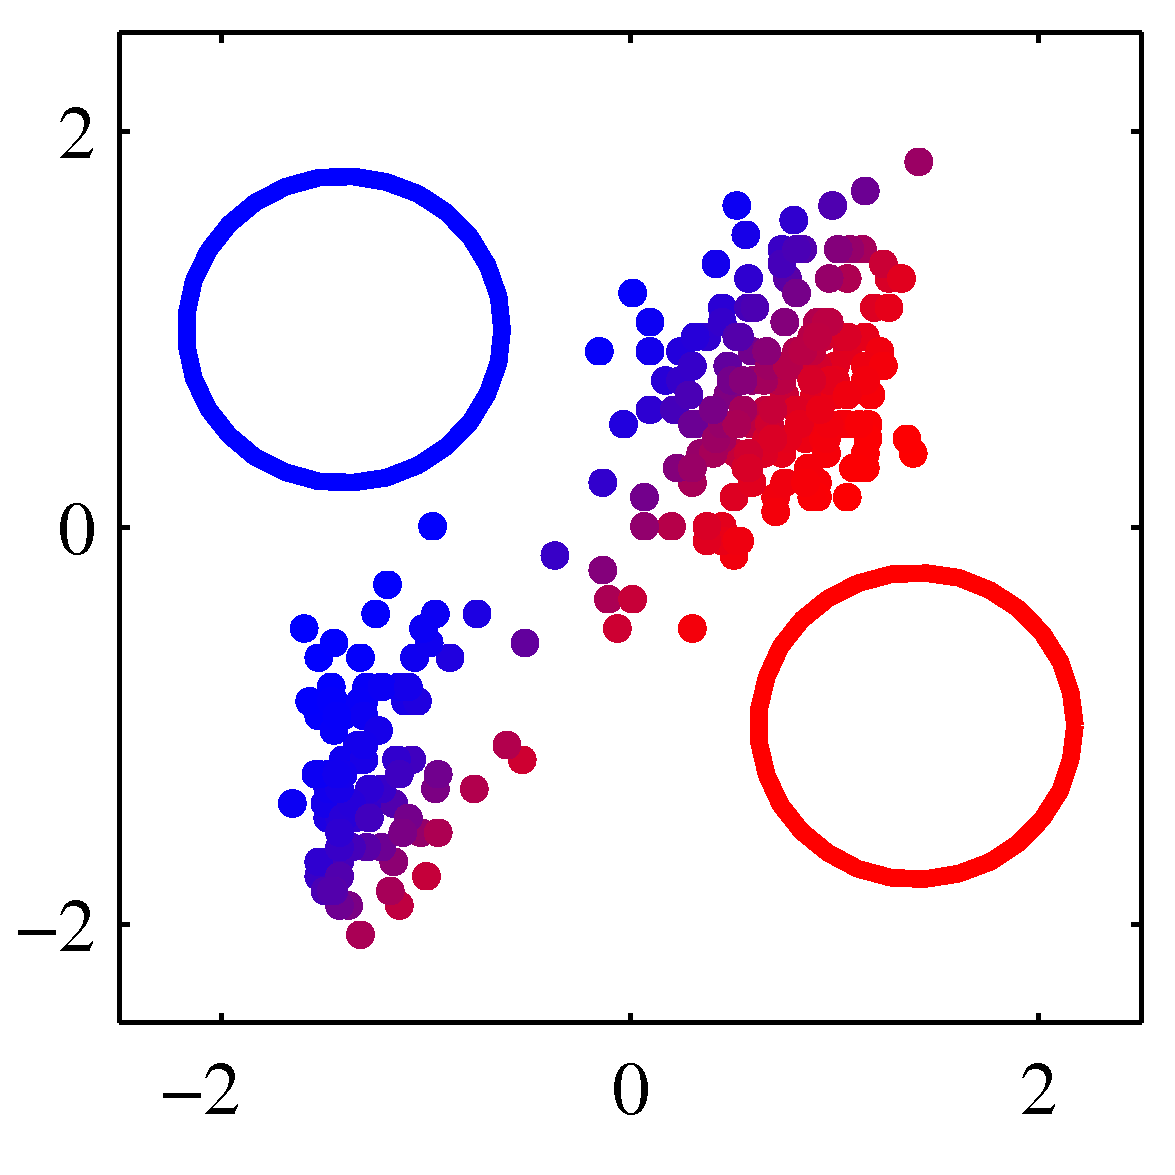
\includegraphics[width=0.25\textwidth]{GMM1}
\caption{Old Faithful data. GMM stared at an abitrary point}
\label{fig:GMM1}
\end{figure}

In Figure \ref{fig:GMM1} above the EM has just started from an arbitrary starting point.
Data shows two apparent clusters, so the model is generated with two components.
The data points are colored by association with the model components.
Note the fading in colors showing strength of relation to model component.
At this point the GMM does not fit data very well.

\begin{figure}[H]
\centering
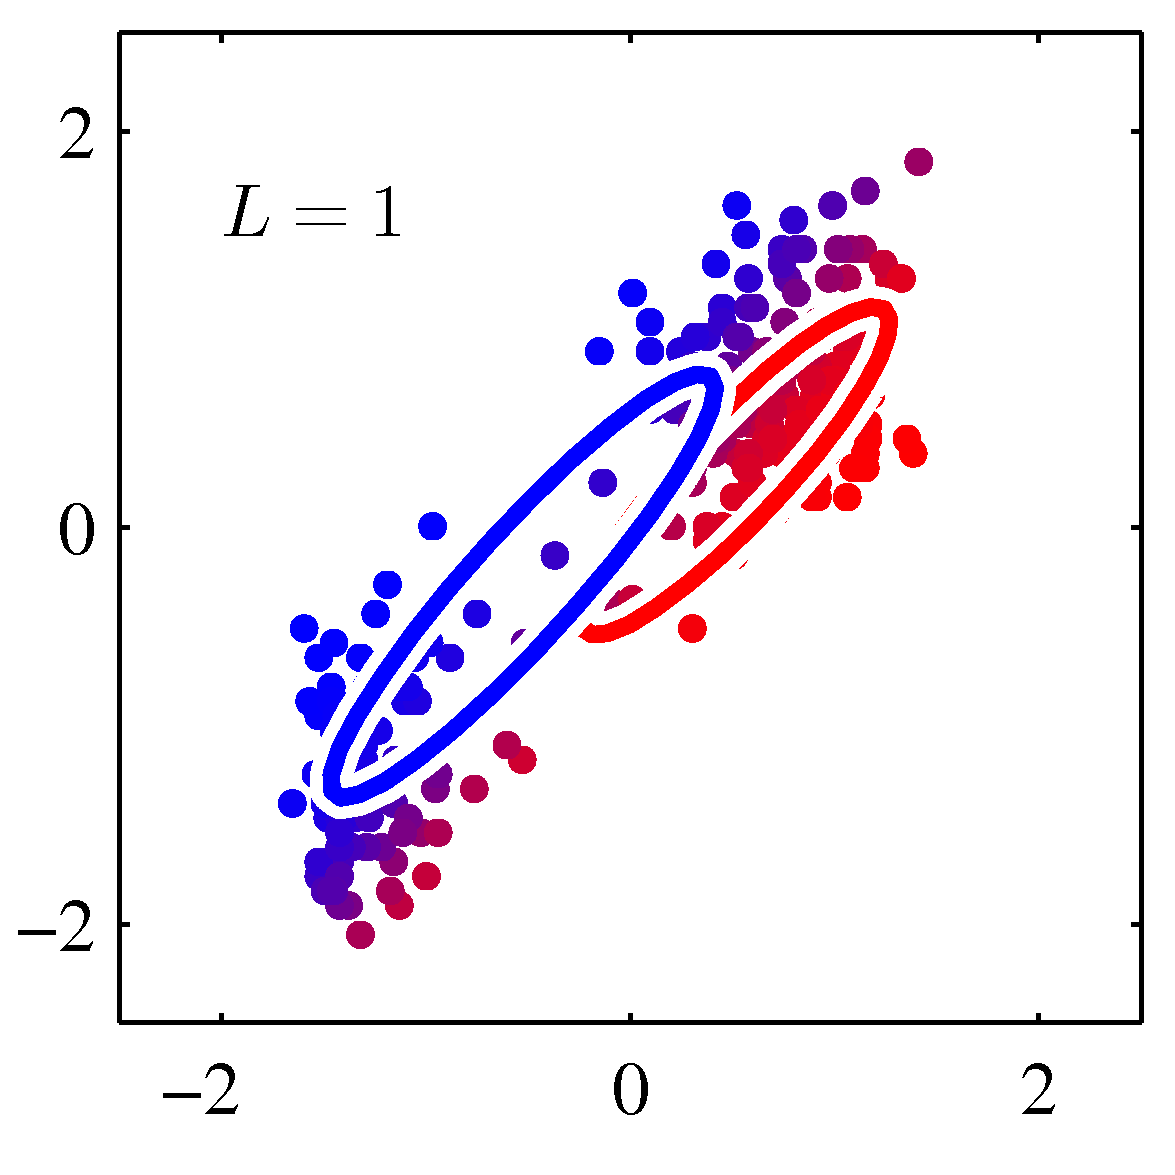
\includegraphics[width=0.25\textwidth]{GMM2}
\caption{Old Faithful data. GMM after one iteration of EM}
\label{fig:GMM2}
\end{figure}

\begin{figure}[H]
\centering
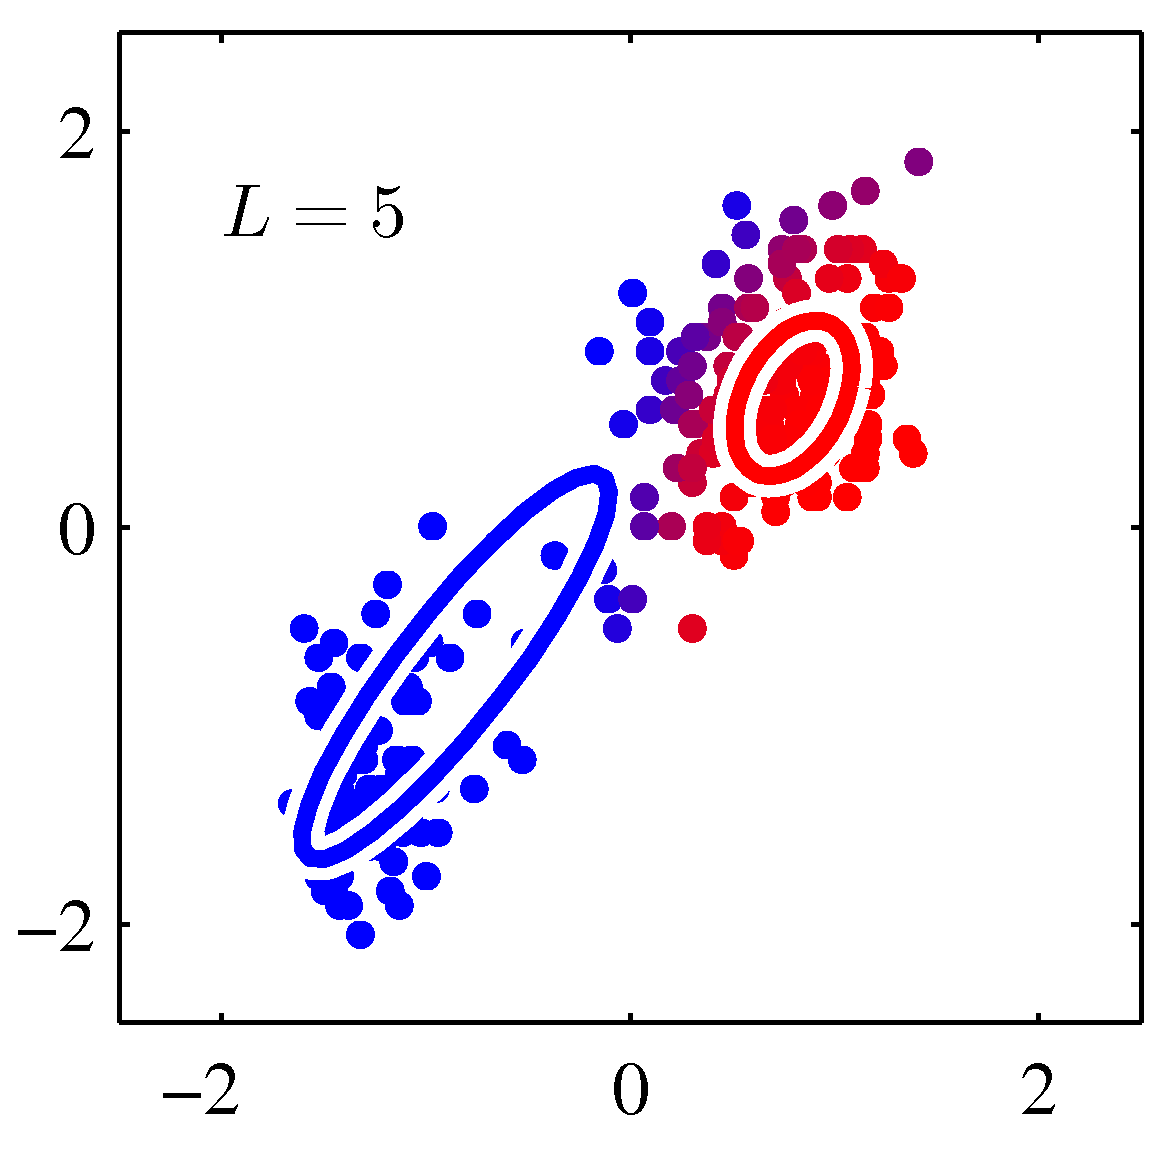
\includegraphics[width=0.25\textwidth]{GMM3}
\caption{Old Faithful data. GMM after five iterations of EM}
\label{fig:GMM3}
\end{figure}

After five iterations the EM has honed in on the centers of the two clusters (Figure \ref{fig:GMM3}).
Note that K-means could have reached roughly this point in as many iterations, but at much less computational cost.

\begin{figure}[H]
\centering
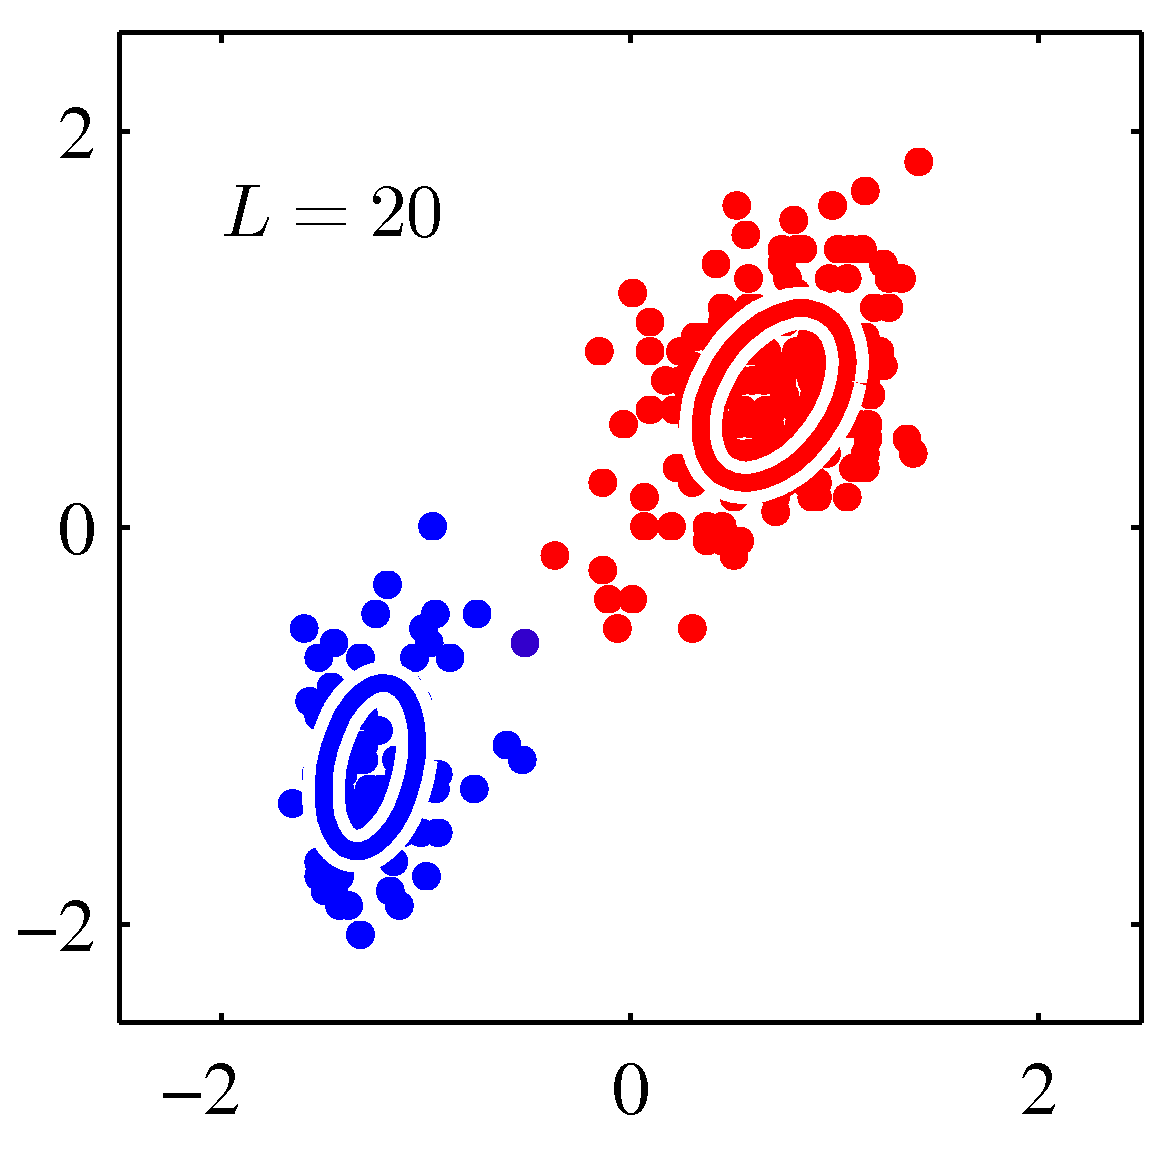
\includegraphics[width=0.25\textwidth]{GMM4}
\caption{Old Faithful data. GMM after 20 iterations of EM}
\label{fig:GMM4}
\end{figure}

As seen in Figure \ref{fig:GMM4} above the model has converged on a well-fitting model after 20 iterations.
This means that further iterations would be superfluous, as they would yield only negligible increases in overall likelihood of the GMM. 


 % Done (-discussion)

%Support Vector Machines - MANGLER 
\chapter{Support Vector Machines}
\section{Theory}

In this section of the appendix the soft margin support vector machine (SVM) is described. The SVM is a binary classifier, which is a problem with multi class. 
The solution for multiclass classification is using a one-vs.-one setup.
With only three classes this is achieved with relative ease. 
The integrated MATLAB statistic toolbox was used to process the data in the SVM case. 

SVM classify by making a decision boundary that maximizes the margin $ \gamma $.
The margin is the perpendicular distance from the decision boundary to the closest feature point.
The standard SVM have a linear decision boundary, which classifies by assigning the new data point to either class $ t=1 $ or $ t=-1 $. 
The decision function for a standard SVM for a test point $ x_{new} $ given by
\begin{equation}
t_{new} = \mathtt{sign}(\mathbf{w}^T \mathbf{x}_{new} +b)
\label{eq:SVM_lin}
\end{equation}
The parameter vector $ \mathbf{w} $ is found by maximizing the margin or minimizing the length of the parameter vector, because of the inverse relationship $ \gamma = \frac{1}{\|\mathbf{w}\|} $.
Moving one single data point can have a huge influence on the position of the decision boundary, The reason is in the constrain
\begin{equation}
t_n(\mathbf{w}^T \mathbf{x}_n + b) \geq 1
\end{equation}   
This however means that all the training features have sit on the correct side of the decision boundary.
This way of classifying is called hard margin SVM, which can't handle overlapping classes.
Therefore a slack to the constrains is introduced $ \xi_n $
 
 
\section{Method}
Radial basis function (gauss med samme variance i alle retninger) 
\section{Results}

\begin{figure}[H]
\centering
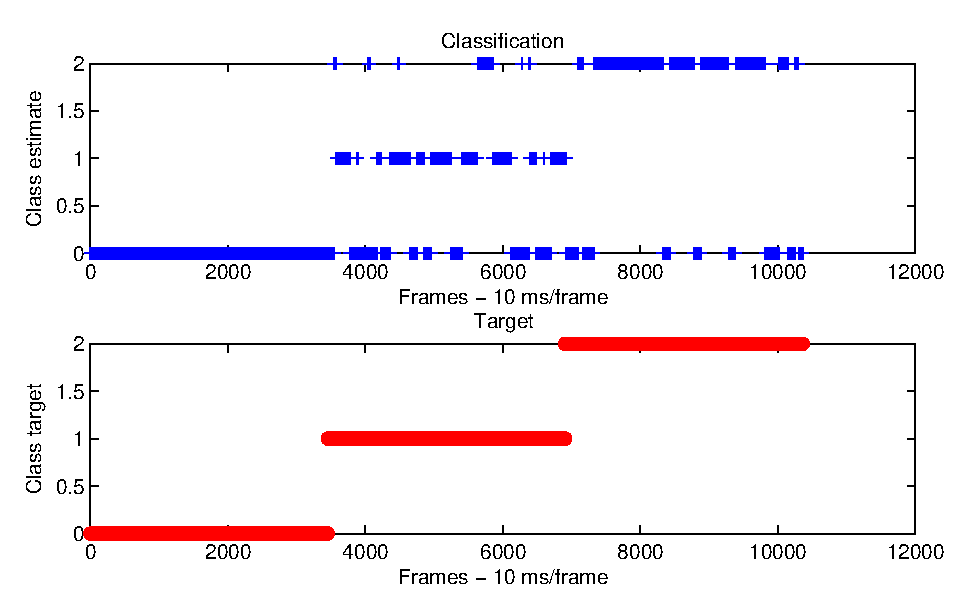
\includegraphics{SVM_3_1digit_PCA10}
\caption{Results of using SVM classifiers and one digit spoken}
\label{fig:SVM3_1dig_PCA}
\end{figure}

\begin{table}[H]                                                    
\centering                                                          
\begin{tabular}{|l|c|c|c|c|}                                        
\hline                                                              
  & Speaker Jacob & Speaker Mose & Speaker Simon & Precision [\%] \\
\hline                                                              
Estimate Jacob & 3454.0 & 1408.0 & 1002.0 & 58.9 \\                 
\hline                                                              
Estimate Mose & 0.0 & 1746.0 & 12.0 & 99.3 \\                       
\hline                                                              
Estimate Simon & 0.0 & 300.0 & 2440.0 & 89.1 \\                     
\hline                                                              
Sensitivity [\%] & 100.0 & 50.6 & 70.6 & 73.7 \\                    
\hline                                                              
\end{tabular}                                                       
\caption{Confusion matrix - 1 digit}                                
\label{table:SVM_3_conf_1}                                          
\end{table} 


\section{Discussion}

% Hidden Markov Models - MANGLER theory and reasons to dump it
\chapter{Hidden Markov Models}
In this project the Hidden Markov models (HMM) is not used on the data.
The reason for this is that the HMM is optimized for recognizing the sequence of the sounds which combines to a word.
HMM is focused on speech recognition and not speaker recognition, which is this project works with.

\section{Theory}   
The HMM is developed to process sequential information in the data, in other models the features have been treated as independent and identical distribution.
When classifying speech from a sequence of data recorded over time, the features tend to be strongly associate with the previous features.
The associated features can be exploited by the HMM to classify.          


\bibliographystyle{ieeetr}
\renewcommand{\bibname}{9 Reference Document}
\addcontentsline{toc}{chapter}{2 Reference Document}
\bibliography{10731@post.au.dk-RefList}

\end{document}          
